% Figure: Trust boundary diagram
\begin{figure}[t]
\centering
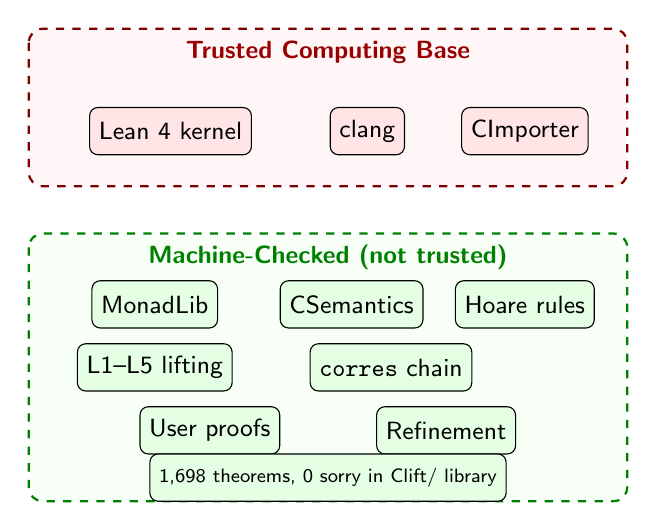
\begin{tikzpicture}[
  trusted/.style={draw, rounded corners=3pt, fill=red!10,
                  minimum height=0.6cm, font=\small\sffamily},
  verified/.style={draw, rounded corners=3pt, fill=green!10,
                   minimum height=0.6cm, font=\small\sffamily},
  label/.style={font=\small\bfseries\sffamily},
]
  % TCB box
  \draw[draw=red!50!black, fill=red!3, rounded corners=5pt, dashed, thick]
    (-3.8, 2.8) rectangle (3.8, 0.8);
  \node[label, text=red!60!black] at (0, 2.5) {Trusted Computing Base};

  \node[trusted] at (-2.0, 1.5) {Lean 4 kernel};
  \node[trusted] at (0.5, 1.5) {clang};
  \node[trusted] at (2.5, 1.5) {CImporter};

  % Verified box
  \draw[draw=green!50!black, fill=green!3, rounded corners=5pt, dashed, thick]
    (-3.8, 0.2) rectangle (3.8, -3.2);
  \node[label, text=green!50!black] at (0, -0.1) {Machine-Checked (not trusted)};

  \node[verified] at (-2.2, -0.7) {MonadLib};
  \node[verified] at (0.3, -0.7) {CSemantics};
  \node[verified] at (2.5, -0.7) {Hoare rules};
  \node[verified] at (-2.2, -1.5) {L1--L5 lifting};
  \node[verified] at (0.8, -1.5) {\texttt{corres} chain};
  \node[verified] at (-1.5, -2.3) {User proofs};
  \node[verified] at (1.5, -2.3) {Refinement};
  \node[verified] at (-0.0, -2.9) {\scriptsize 1,698 theorems, 0 sorry in Clift/ library};

\end{tikzpicture}
\caption{Trust boundary. Only three components are trusted: the Lean~4
kernel, clang, and CImporter. All proofs, lifting stages, and Hoare
rules are machine-checked.}
\label{fig:trust}
\end{figure}
